\begin{frame}
  \frametitle{1D Chain of Atoms --- 1 Atom per Unit}
  A 1D chain of $N$ equally spaced atoms at $R_j(t)= x_j + u_j(t)$
  \begin{center}
    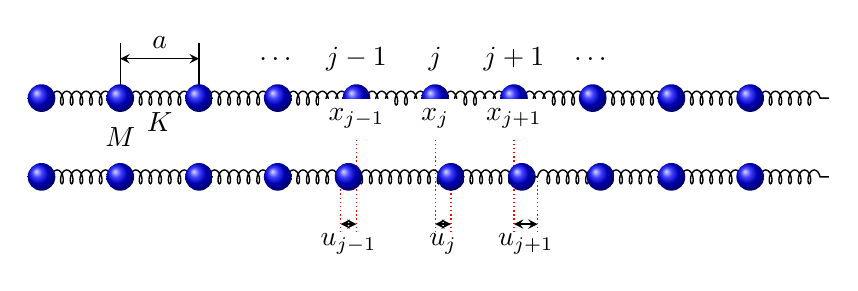
\begin{tikzpicture}
      [
      spring/.style={
        line width=0.5pt,
        decorate,
        decoration={
            coil,
            amplitude=2.5,
            segment length=3.5,
          }
        },
      ]
      \draw[line width=0.5pt] (1.0, 0.0) -- (1.0, 0.7);
      \draw[line width=0.5pt] (2.0, 0.0) -- (2.0, 0.7);
      \draw[line width=0.5pt, <->, >=stealth] (1.0, 0.5) -- node[pos=0.5, anchor=south] {$a$} (2.0, 0.5);

      \node[anchor=center] at (1, -0.5) {$M$};
      \node[] at (1.5,  -0.3) {$K$};

      \node[] at (3.0, 0.5) {\ldots};
      \node[] at (4.0, 0.5) {$j-1$};
      \node[] at (5.0, 0.5) {$j$};
      \node[] at (6.0, 0.5) {$j+1$};
      \node[] at (7.0, 0.5) {\ldots};

      \draw[line width=0.5pt, densely dotted, draw=red] (4.0, -0.0) -- (4.0, -1.7);
      \draw[line width=0.5pt, densely dotted, draw=red] (5.0, -0.0) -- (5.0, -1.7);
      \draw[line width=0.5pt, densely dotted, draw=red] (6.0, -0.0) -- (6.0, -1.7);
      \draw[line width=0.5pt, densely dotted, draw=red] (3.8, -1.0) -- (3.8, -1.7);
      \draw[line width=0.5pt, densely dotted, draw=red] (5.2, -1.0) -- (5.2, -1.7);
      \draw[line width=0.5pt, densely dotted, draw=red] (6.3, -1.0) -- (6.3, -1.7);

      \foreach \x in {0,1,...,9}{
        % draw the spring
        \draw[spring, draw=black] (\x, 0) -- ++(1, 0);
        % draw the atoms
        \ifthenelse{\x > 0}
        {
            \shade[ball color=blue] (\x, 0) circle (5pt);
        }{}
      }


      \foreach \x [remember=\x as \lastx (initially 0)] in {
        0.0, 1.0, 2.0, 3.0, 3.8,
        5.2, 6.3, 7.1, 8.0, 9.0, 10.0
      }
      {
        \ifthenelse{\lengthtest{\x pt > 0 pt}}
        {
          % draw the spring
          \draw[spring, draw=black] (\lastx, -1) -- (\x, -1);
        }{}
      }
      \foreach \x [remember=\x as \lastx (initially 0)] in {
        0.0, 1.0, 2.0, 3.0, 3.9,
        5.2, 6.1, 7.1, 8.0, 9.0
      }
      {
        \ifthenelse{\lengthtest{\x pt > 0 pt}}
        {
          % draw the atoms
          \shade[ball color=blue] (\x, -1) circle (5pt);
        }{}
      }

      \node[below=0.3, anchor=north, fill=white] at (4.0, 0.0) {$x_{j-1}$};
      \node[below=0.3, anchor=north, fill=white] at (5.0, 0.0) {$x_{j}$};
      \node[below=0.3, anchor=north, fill=white] at (6.0, 0.0) {$x_{j+1}$};

      \draw[line width=0.5pt, <->, >=stealth] (4.0, -1.6) -- node[pos=0.5, below, anchor=north] {$u_{j-1}$} (3.8, -1.6);
      \draw[line width=0.5pt, <->, >=stealth] (5.0, -1.6) -- node[pos=0.5, below, anchor=north] {$u_{j}$} (5.2, -1.6);
      \draw[line width=0.5pt, <->, >=stealth] (6.0, -1.6) -- node[pos=0.5, below, anchor=north] {$u_{j+1}$} (6.3, -1.6);
    \end{tikzpicture}
  \end{center}

  The Newton's Equation
  \begin{equation*}
    \label{eq:1d_newton_eq}
    M \frac{\mathrm{d}^2 u_j}{\mathrm{d}t^2}
    % = K (u_{j+1} - u_j) + K (u_{j-1} - u_j)
    = K (u_{j+1} + u_{j-1} - 2u_j)
    \qquad j=1,\ldots,N
  \end{equation*}

  % Where $x_j$ is the deviation from the equilibrium position for the
  % $j$-\textit{th} atom.

  
  Assume the solution has the form $u_j(t) = \frac{A_q}{\sqrt{M}}e^{i(q\mathcolor{red}{x_j} -
    \omega t)}$,
  then
  \footnote{
    $u_j(t)$ here is complex. In practice, take the real part, i.e. $\Re[{u_j(t)}]$.
  }

  \begin{align*}
    \omega^2 &= {K\over M}(2 - e^{iqa} - e^{-iqa}) \cr
               &= {2K\over M} (1 - \cos{qa}) \cr
        \Rightarrow \quad \omega &= \sqrt{4K\over M}\left|\sin{qa\over 2}\right|
  \end{align*}
\end{frame}